\documentclass[12pt,onecolumn,a4paper]{article}

\usepackage{graphicx}
\usepackage{amsthm}
\usepackage{titling}
\usepackage{bigints}
\usepackage{amssymb}
\usepackage{changepage}
\usepackage{booktabs, tabularx, multirow}
\usepackage{tkz-graph}
\usepackage{tikz,amsmath,pgf}
\usepackage{natbib}
\usepackage{listings}
\usepackage{subcaption}
\usepackage[section]{placeins}
\usepackage[legalpaper, margin=1.3in]{geometry}

\graphicspath{ {C:/Users/Sepehr/Desktop/Term 9/AI/Barekati - 610398105 - HW1/Q2/images} }

\definecolor{codegreen}{rgb}{0,0.6,0}
\definecolor{codegray}{rgb}{0.5,0.5,0.5}
\definecolor{codepurple}{rgb}{0.58,0,0.82}
\definecolor{backcolour}{rgb}{0.95,0.95,0.92}

\lstdefinestyle{mystyle}{
    backgroundcolor=\color{backcolour},   
    commentstyle=\color{codegreen},
    keywordstyle=\color{magenta},
    numberstyle=\tiny\color{codegray},
    stringstyle=\color{codepurple},
    basicstyle=\ttfamily\footnotesize,
    breakatwhitespace=false,         
    breaklines=true,                 
    captionpos=b,                    
    keepspaces=true,                 
    numbers=left,                    
    numbersep=5pt,                  
    showspaces=false,                
    showstringspaces=false,
    showtabs=false,                  
    tabsize=1
}

\lstset{style=mystyle}

\begin{document}

\section{Explain what the number of states depends on. Can the number of states be reduced?}
The number of states in this problem depends on several factors:
\begin{enumerate}
	\item{\textbf{Size of the environment:}} The dimensions of the grid directly affect the number of possible states. In the given environment, the size of the grid is 7x9, which means there are 63 cells in total.
	\item{\textbf{Number of dots:}} Each dot can either be present or absent in each cell, so the number of dots on the grid contributes to the total number of states. In the given environment, there are 15 dots.
	\item{\textbf{Number of walls:}} Walls restrict the movement of the agent, so their placement affects the reachable states. More walls generally reduce the number of reachable states by limiting the agent's movement options.
	\item{\textbf{Number of ghosts (optional):}} If ghosts are included in the environment, their positions also affect the reachable states because the agent must avoid them.
	\item{\textbf{Starting position of the agent:}} The agent's starting position is also a factor, as it determines the initial state from which the agent begins its exploration.
\end{enumerate}
To reduce the number of states, several strategies can be employed:
\begin{enumerate}
\item{\textbf{Symmetry and Redundancy Removal:}} If there are symmetrical patterns in the environment, states that are symmetrical to each other can be merged to reduce redundancy.
\item{\textbf{Dynamic Programming and Memoization:}} If certain states lead to the same outcomes, those states can be combined or memoized to avoid redundant computations.
\item{\textbf{State Abstraction:}} Instead of considering each cell individually, certain groups of cells with similar characteristics can be abstracted into a single state, reducing the overall state space.
\item{\textbf{Heuristic Search:}} Use heuristics to guide the search process towards promising areas of the state space, thereby reducing the number of explored states.
\item{\textbf{State Pruning:}} Certain states might be unreachable or irrelevant to the problem's goal. Identifying and pruning such states can help reduce the state space.
\end{enumerate}

\section{Define Action, State, Rewards, and Goal State for the problem and provide your explanation.}
\begin{enumerate}
	\item{\textbf{Action:}} Actions are the possible moves that the agent can take in the environment. In this problem, the agent can typically move in four directions: up, down, left, and right. However, the agent's movement might be restricted by walls, and it must avoid ghosts. Therefore, the set of actions might vary depending on the current state of the environment. Actions can be represented as integers or symbols corresponding to movement directions, such as 0 for up, 1 for down, 2 for left, and 3 for right.
	\item{\textbf{State:}} The state represents the configuration of the environment at a given point in time. It includes the positions of the agent, dots, walls, and ghosts. In this problem, a state can be represented as a grid where each cell contains information about whether it's empty, contains a dot, is occupied by a wall, the agent, or a ghost.
	\item{\textbf{Rewards:}} Rewards are numerical values assigned to the agent based on its actions and the resulting states. In this problem, we can define the following reward scheme:
	\begin{itemize}
		\item{\textbf{Collecting a dot:}} +1 reward
		\item{\textbf{Touching a ghost:}} -1 reward (penalty)
		\item{\textbf{Moving into a wall:}} -1 reward (penalty)
		\item{\textbf{Reaching the goal state:}} +10 reward (or any positive value indicating successful completion)
	\end{itemize}
	\item{\textbf{Goal State:}} The goal state represents the desired configuration of the environment that indicates the successful completion of the task. In this problem, the goal state is reached when all dots have been collected by the agent without touching any ghosts. Once all dots are collected, the environment is considered to be in a goal state, and the agent has completed its task successfully.
\end{enumerate}

\section{First, consider the environment as shown above. Analyze the effect of $\gamma$ for at least 3 gamma values equal to 0.25, 0.5, and 1. Also, for at least 3 $\alpha$ values, analyze the results and determine the impact of $\alpha$.}
In reinforcement learning, $\gamma$ (gamma) is the discount factor and $\alpha$ (alpha) is the learning rate. Let's analyze the effect of different values of $\gamma$ and $\alpha$ on the agent's learning and decision-making process in the given environment.\\

\subsection*{Effect of $\gamma$:}
\begin{enumerate}
	\item{\textbf{$\gamma = 0.25$ (Low Discount Factor):}}
	\begin{itemize}
		\item With a low discount factor, the agent heavily discounts future rewards. It prioritizes immediate rewards over long-term rewards.
		\item The agent's actions are more influenced by the immediate consequences rather than considering future states.
		\item This might lead to myopic behavior where the agent focuses on short-term gains without considering the overall goal.
		\item In the given environment, the agent might prioritize collecting nearby dots and avoiding ghosts without considering the long-term strategy of collecting all dots efficiently.
	\end{itemize}
	\item{\textbf{$\gamma = 0.5$ (Moderate Discount Factor):}}
	\begin{itemize}
		\item A moderate discount factor balances the importance of immediate rewards and future rewards.
		\item The agent considers both short-term gains and long-term goals in its decision-making process.
		\item It strikes a balance between exploration and exploitation, exploring new states while also exploiting known good actions.
		\item In the given environment, the agent would still prioritize nearby dots and avoid ghosts, but with some consideration for the overall goal of collecting all dots.
	\end{itemize}
	\item{\textbf{$\gamma = 1$ (High Discount Factor):}}
	\begin{itemize}
		\item With a high discount factor, the agent values future rewards almost as much as immediate rewards.
		\item The agent takes a more long-term approach, considering future states and rewards extensively in its decision-making process.
		\item It focuses on maximizing cumulative rewards over time, even if it means sacrificing immediate gains.
		\item In the given environment, the agent would plan its actions strategically to efficiently collect all dots while avoiding ghosts, considering the long-term consequences of its actions.
	\end{itemize}
\end{enumerate}

\subsection*{Effect of $\gamma$:}
\begin{enumerate}
	\item{\textbf{Low $\alpha$}}
	\begin{itemize}
		\item With a low learning rate, the agent updates its Q-values slowly.
		\item It gives more weight to past experiences and is less influenced by new information.
		\item The learning process is slow, and the agent requires more iterations to converge to an optimal policy.
		\item In the given environment, the agent's behavior might be more conservative, as it relies heavily on its initial Q-value estimates and past experiences.
	\end{itemize}
	\item{\textbf{Moderate $\alpha$}}
	\begin{itemize}
		\item A moderate learning rate balances between exploiting new information and maintaining stability.
		\item The agent updates its Q-values at a moderate pace, incorporating new experiences while also retaining valuable knowledge from past experiences.
		\item It converges to an optimal policy faster compared to a low learning rate.
		\item In the given environment, the agent learns from both successes and failures, gradually improving its strategy over time.
	\end{itemize}
	\item{\textbf{High $\alpha$}}
	\begin{itemize}
		\item With a high learning rate, the agent updates its Q-values rapidly.
		\item It gives more weight to recent experiences and is highly influenced by new information.
		\item The learning process is fast, and the agent adapts quickly to changes in the environment.
		\item In the given environment, the agent might exhibit more exploratory behavior, as it readily incorporates new information into its decision-making process, potentially leading to faster convergence to an optimal policy.
	\end{itemize}
\end{enumerate}

\section{ Display the environment as a weighted graph. The vertices of different modes and their weights are the amount of Reward after applying the corresponding Action. You can mention the corresponding Action as a Label on each edge.}

\begin{lstlisting}[language=Python]
# Weighted Graph
import networkx as nx
import matplotlib.pyplot as plt

# Define the environment as a grid
board = [
    ['A', 'D', 'D', 'D', 'D', 'D', 'D', 'D', 'D'],
    ['D', 'W', 'W', 'W', 'D', 'W', 'W', 'W', 'D'],
    ['D', 'W', 'D', 'D', 'D', 'D', 'D', 'W', 'D'],
    ['D', 'D', 'D', 'W', 'E', 'W', 'D', 'D', 'D'],
    ['D', 'W', 'D', 'W', 'G', 'W', 'D', 'W', 'D'],
    ['D', 'W', 'D', 'D', 'W', 'D', 'D', 'W', 'D'],
    ['D', 'D', 'D', 'D', 'D', 'D', 'D', 'D', 'D']
]

# Create a weighted graph
G = nx.Graph()

# Add vertices (nodes) representing each cell in the grid
for i in range(len(board)):
    for j in range(len(board[0])):
        G.add_node((i, j))

# Define actions and their corresponding rewards
actions = {
    (0, 1): 1,  # Up
    (0, -1): -1,  # Down
    (-1, 0): -1,  # Left
    (1, 0): -1  # Right
}

# Add edges representing actions with their corresponding rewards
for i in range(len(board)):
    for j in range(len(board[0])):
        if board[i][j] != 'W':  # Ignore walls
            for action, reward in actions.items():
                new_i, new_j = i + action[0], j + action[1]
                if (0 <= new_i < len(board) and 0 <= new_j < len(board[0]) and
                        board[new_i][new_j] != 'W'):  # Ensure not to go out of bounds or onto walls
                    G.add_edge((i, j), (new_i, new_j), weight=reward, action=action)

# Draw the graph
pos = {(i, j): (j, -i) for i in range(len(board)) for j in range(len(board[0]))}  # Position vertices
nx.draw(G, pos, with_labels=True, node_size=700, node_color='lightblue', font_size=8, font_weight='bold')
edge_labels = {(u, v): f"{d['weight']} ({d['action']})" for u, v, d in G.edges(data=True)}
nx.draw_networkx_edge_labels(G, pos, edge_labels=edge_labels)
plt.title("Weighted Graph representing the Environment")
plt.gca().invert_yaxis()  # Invert y-axis to match grid coordinates
plt.show()
\end{lstlisting}

The code is in .ipynb file and the result is shown in both Q-table and Graph.pdf file and .ipynb file.

\section{ Draw the Q-Table for this problem.}
\begin{lstlisting}[language=Python]
# Q-Table
import numpy as np

# Define the dimensions of the grid
num_rows = 7
num_cols = 9
num_actions = 4  # Up, Down, Left, Right

# Initialize the Q-Table with zeros
q_table = np.zeros((num_rows, num_cols, num_actions))

# Display the Q-Table
print("Q-Table:")
print("State | Action: 0 (Up) | Action: 1 (Down) | Action: 2 (Left) | Action: 3 (Right)")
print("-" * 81)
for i in range(num_rows):
    for j in range(num_cols):
        row_str = f"({i},{j})  |"
        for k in range(num_actions):
            row_str += f"  q({i},{j},{k}): {q_table[i, j, k]:.2f}  |"
        print(row_str)
\end{lstlisting}

The code is in .ipynb file and the result is shown in both Q-table and Graph.pdf file and .ipynb file.

\section{Test your code on another arbitrary environment and report the result.}
\begin{lstlisting}[language=Python]
import numpy as np
import random

# Define the environment as a grid
board = [
    ['A', 'D', 'D', 'D', 'D', 'D', 'D', 'D', 'D'],
    ['D', 'W', 'W', 'W', 'D', 'W', 'W', 'W', 'D'],
    ['D', 'w', 'D', 'D', 'D', 'D', 'D', 'W', 'D'],
    ['D', 'D', 'D', 'W', 'E', 'W', 'D', 'D', 'D'],
    ['D', 'W', 'D', 'W', 'G', 'W', 'D', 'W', 'D'],
    ['D', 'W', 'D', 'D', 'W', 'D', 'D', 'W', 'D'],
    ['D', 'D', 'D', 'D', 'D', 'D', 'D', 'D', 'D']
]

# Define actions and their corresponding indices
actions = {
    'up': 0,
    'down': 1,
    'left': 2,
    'right': 3
}

# Define rewards for actions
rewards = {
    1: 1,  # Dot collected
    -1: -1,  # Wall or ghost
    10: 10  # Goal state reached
}

# Initialize Q-Table with zeros
q_table = np.zeros((len(board), len(board[0]), len(actions)))

# Define epsilon-greedy policy parameters
epsilon = 0.1
alpha = 0.1
gamma = 0.9

# Convert the board into a numpy array
board = np.array(board)

# Define helper functions
def get_possible_actions(state):
    """Get possible actions from a given state."""
    possible_actions = []
    for action, idx in actions.items():
        new_state = get_new_state(state, idx)
        if is_valid_move(new_state):
            possible_actions.append(idx)
    return possible_actions

def get_new_state(state, action_idx):
    """Get the new state after taking an action."""
    action = list(actions.keys())[action_idx]
    if action == 'up':
        return (state[0] - 1, state[1])
    elif action == 'down':
        return (state[0] + 1, state[1])
    elif action == 'left':
        return (state[0], state[1] - 1)
    elif action == 'right':
        return (state[0], state[1] + 1)

def is_valid_move(state):
    """Check if a move is valid."""
    x, y = state
    return 0 <= x < len(board) and 0 <= y < len(board[0]) and board[x, y] != 'W'

def choose_action(state):
    """Choose an action using epsilon-greedy policy."""
    if np.random.rand() < epsilon:
        return random.choice(get_possible_actions(state))
    else:
        return np.argmax(q_table[state[0], state[1]])

# Main loop
start_state = (0, 0)  # Starting state
current_state = start_state
goal_state = (3, 4)  # Define the goal state
while 'D' in board.flatten():
    action_idx = choose_action(current_state)
    action = list(actions.keys())[action_idx]
    new_state = get_new_state(current_state, action_idx)
    if is_valid_move(new_state):
        reward = rewards[1] if board[new_state] == 'D' else rewards[-1]
        q_table[current_state[0], current_state[1], action_idx] += alpha * (reward + gamma * np.max(q_table[new_state]) - q_table[current_state[0], current_state[1], action_idx])
        board[current_state] = 'E'  # Mark current position as empty
        board[new_state] = 'A'  # Move the agent to the new position
        current_state = new_state

        # Display the board
        for row in board:
            print(' '.join(row))
        print()

        input("Press Enter to continue...")
    else:
        print("Invalid move. Try another action.")

print("No more dots left. Goal state reached!")
\end{lstlisting}
Must run to see the result, but at the end it gives \textbf{No more dots left. Goal state reached!}.\\
\begin{center}
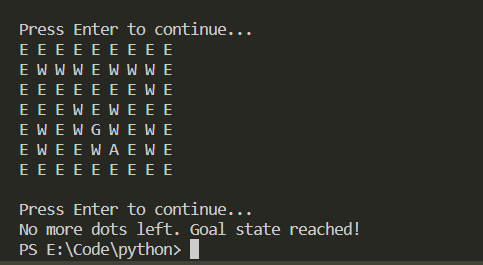
\includegraphics{Result}
\end{center}
\end{document}



